%\documentclass[letterpaper, 10 pt, conference]{ieeeconf}
%\usepackage{filecontents,lipsum}
%\usepackage[noadjust]{cite}
%%\begin{filecontents*}{references.bib}
%%@article{Khoe:1994:CML:2288694.2294265,
%%    author = {Khoe, G. -D.},
%%    title = {Coherent multicarrier lightwave technology for flexible capacity networks},
%%    journal = {Comm. Mag.},
%%    issue_date = {March 1994},
%%    volume = {32},
%%    number = {3},
%%    month = mar,
%%    year = {1994},
%%    issn = {0163-6804},
%%    pages = {22--33},
%%    numpages = {12},
%%    url = {http://dx.doi.org/10.1109/35.267438},
%%    doi = {10.1109/35.267438},
%%    acmid = {2294265},
%%    publisher = {IEEE Press},
%%    address = {Piscataway, NJ, USA},
%%}
%%\end{filecontents*}
%\title{This document}
%\author{This author}

%%%%%%%%%%%%%%%%%%%%%%%%%%%%%%%%%%%%%%%%%%%%%%%%%%%%%%%%%%%%%%%%%%%%%%%%%%%%%%%%
%2345678901234567890123456789012345678901234567890123456789012345678901234567890
%        1         2         3         4         5         6         7         8

\documentclass[letterpaper, 10 pt, conference]{ieeeconf}  % Comment this line out if you need a4paper

%\documentclass[a4paper, 10pt, conference]{ieeeconf}      % Use this line for a4 paper

\IEEEoverridecommandlockouts                              % This command is only needed if 
                                                          % you want to use the \thanks command

\overrideIEEEmargins                                      % Needed to meet printer requirements.

% See the \addtolength command later in the file to balance the column lengths
% on the last page of the document

% The following packages can be found on http:\\www.ctan.org
%\usepackage{graphics} % for pdf, bitmapped graphics files
%\usepackage{epsfig} % for postscript graphics files
%\usepackage{mathptmx} % assumes new font selection scheme installed
%\usepackage{times} % assumes new font selection scheme installed
%\usepackage{amsmath} % assumes amsmath package installed
%\usepackage{amssymb}  % assumes amsmath package installed
%\usepackage{filecontents,lipsum}
%\usepackage[noadjust]{cite}
%\usepackage{bm}
%\usepackage{tikz}
%\usepackage{graphicx}
%\usepackage{caption}
%\usepackage{subcaption}
%\usepackage{multicol}
%\usepackage{url}
%\usepackage{geometry}
%\usepackage{mathtools}
%\usepackage[utf8]{inputenc}
%\usepackage[english]{babel}
%\usepackage{algorithm}
%\usepackage[]{algpseudocode}


\usepackage{afterpage}
\usepackage{algorithm}
\usepackage[]{algpseudocode}
\usepackage{amsmath}
\usepackage{amssymb}  % assumes amsmath package installed
\usepackage{arydshln}
\usepackage[english]{babel}
\usepackage{bm}
\usepackage{caption}
\usepackage[T1]{fontenc}
\usepackage{graphicx}
\usepackage[utf8]{inputenc}
\usepackage{multicol}
\usepackage[T1]{xcolor}
\usepackage{soul}
\usepackage{subfig}
\usepackage{tikz}
\usepackage{url}
\usepackage[backend=biber,style=ieee,sorting=none]{biblatex}
\addbibresource{bib/references.bib}

\newcommand\blankpage{%
    \null
    \thispagestyle{empty}%
    \addtocounter{page}{-1}%
    \newpage}



\newcommand*{\important}[1]{\textcolor{red}{\danger~\textbf{IMPORTANT:~}} \textcolor{red}{#1}}

\newcommand*{\pending}[1]{\textcolor{blue}{$\bigstar$~\textbf{PENDING~#1}}}

\newcommand\mybox[2][]{\tikz[overlay]\node[fill=blue!100,inner sep=4pt, anchor=text, rectangle, rounded corners=1mm,#1] {#2};\phantom{#2}}

\newcommand{\TODO}{\mybox[fill=yellow]{\textcolor{blue}{\Large \textbf{TODO}}}}

\newtheorem{prop}{Proposition}

\title{\LARGE \bf
Dynamic sensorimotor graphs
}


\author{Some Guy, Nice Dude}

\begin{document}

\maketitle

\begin{abstract}
Regularities present in the sensorimotor signals of a robotic agent can reflect its embodiment, as well as the associations resulting from the active control policy. In this work, we analyze the functional connectivity of the sensorimotor signals based on pairwise mutual information. As the robot performs exploratory motions based on motor babbling we capture and study the time-varying changes in the relationships. We provide analysis of the instantaneous and average sharing of information and extrapolate the meaning in relation to the physical properties of the robot's body. Results from a simulated planar system validate the use of mutual information as a tool not only for the analysis of the relationships between the sensorimotor signals but also to drive exploratory motions.
\TODO
\end{abstract}
% =============================================================================
%                                                                             |
%                                                                             |
% ------------------------------- SECTION ------------------------------------|
%                                                                             |
%                                                                             |
% =============================================================================
\section{Introduction}\label{sec:intro}
\TODO
\begin{figure}[!th]
	\centering
	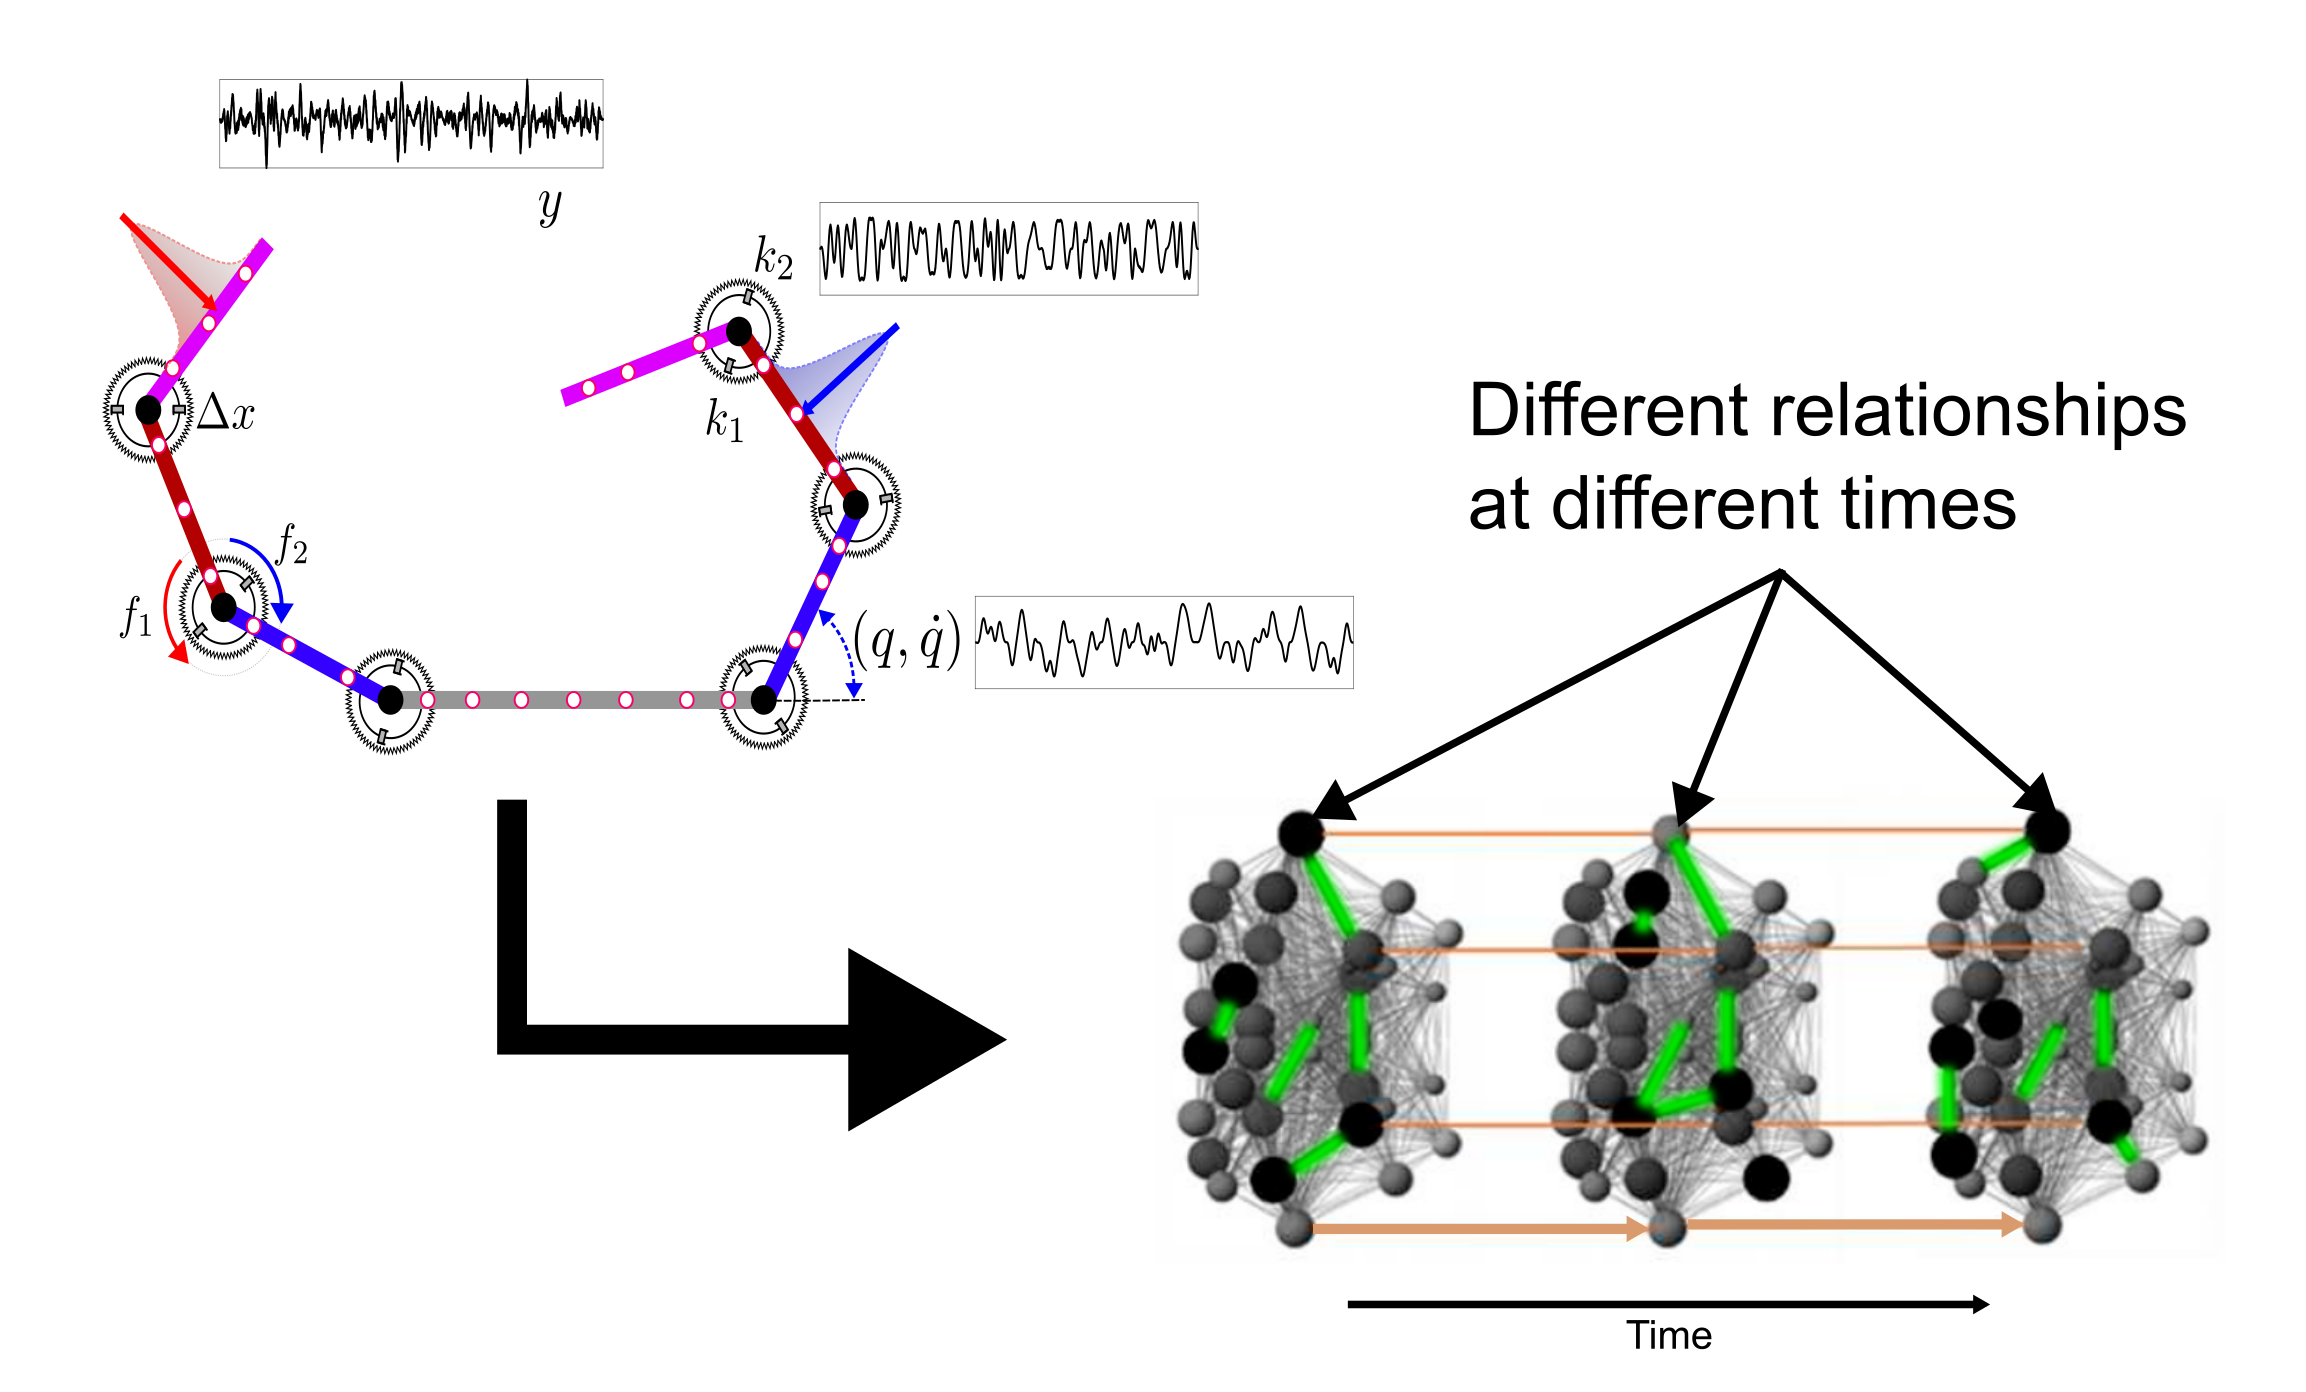
\includegraphics[width=0.9\columnwidth]{fig/general_overview.png}
	\caption{General overview.}
	\label{fig:general_overview}
\end{figure}


% SUBSECTION ==================================================================
\subsection{Related works}

Refer to Mannella, Gama, Marcel, Kanazawa, Husbands, Hoffmann (puppy).

% SUBSECTION ==================================================================
\subsection{Contributions}
\TODO
In this work we present an analysis based on the information theory of the dnyamic relationships exsiting among the sensorimotor signals of a robot. In the analysis we show how the amount of information sharing in the system is related to the motion of the robot and the tactile events that occur duting motion. Furthermore, using nonnegative matrix factoriztion we identify operation modes of the robot based only of the mutual information measurments. In a case study we demonstrate how by only foucsing on the mutual information and without having knowledge about the morphology of the robot, an excitation trajectory can be devised that avoids self contact. A comparison of this trajectory against conventional trajevetory design methods is presented.

% =============================================================================
%                                                                             |
%                                                                             |
% ------------------------------- SECTION ------------------------------------|
%                                                                             |
%                                                                             |
% =============================================================================
\section{The robot model}
\TODO

\begin{figure}[!th]
	\centering
	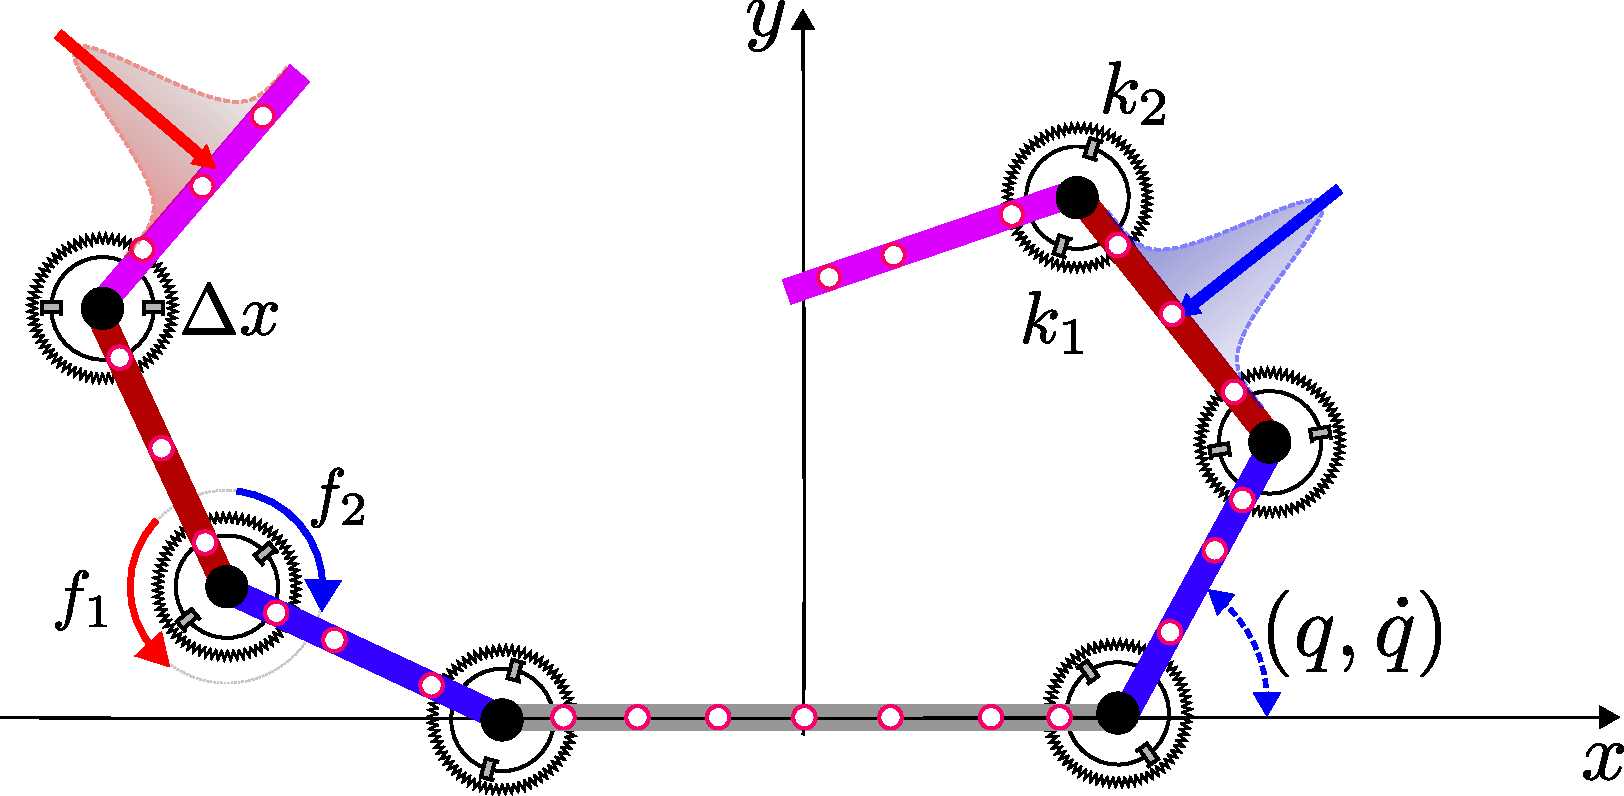
\includegraphics[width=0.9\columnwidth]{fig/extended_dual_arm_robot.pdf}
	\caption{The planar dual arm robot.}
	\label{fig:extended_dual_arm_robot}
\end{figure}
% =============================================================================
%                                                                             |
%                                                                             |
% ------------------------------- SECTION ------------------------------------|
%                                                                             |
%                                                                             |
% =============================================================================
\section{Graph decomposition}
\TODO

\begin{figure}[!th]
	\centering
	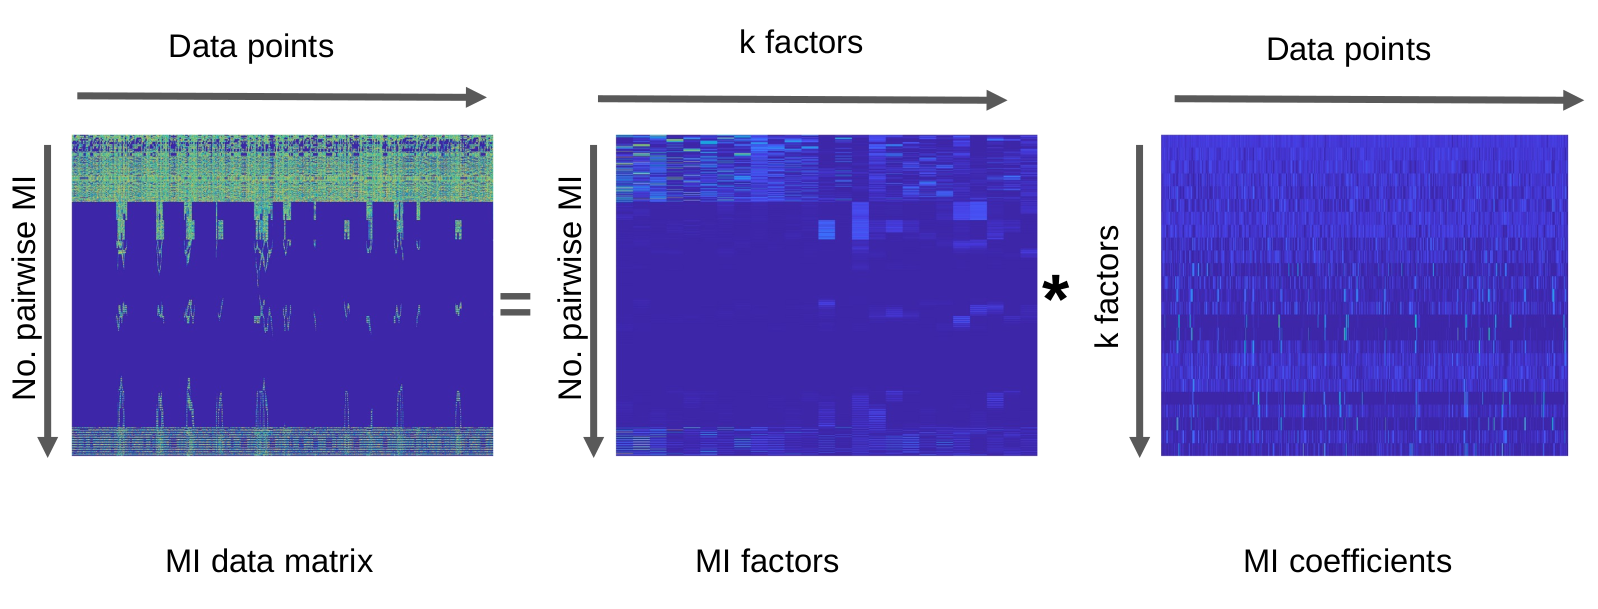
\includegraphics[width=0.9\columnwidth]{fig/nnmf.png}
	\caption{Decomposition of the mutual information data matrix using non negative matrix factorization.}
	\label{fig:nnmf}
\end{figure}

% =============================================================================
%                                                                             |
%                                                                             |
% ------------------------------- SECTION ------------------------------------|
%                                                                             |
%                                                                             |
% =============================================================================
\section{Simulation results}
\TODO

% =============================================================================
%                                                                             |
%                                                                             |
% ------------------------------- SECTION ------------------------------------|
%                                                                             |
%                                                                             |
% =============================================================================
\section{Case study: robot excitation trajectories}
\TODO
In this section we use the instantaneous mutual information to generate trajectories for the left and right arms avoiding potential collisions. This is done agnostic to the actual morphology of the robot. In contrast we use a standard method for the design of excitation trajectories and compare the results.

% =============================================================================
%                                                                             |
%                                                                             |
% ------------------------------- SECTION ------------------------------------|
%                                                                             |
%                                                                             |
% =============================================================================
\section{Beyond robotics}
\TODO

% =============================================================================
%                                                                             |
%                                                                             |
% ------------------------------- SECTION ------------------------------------|
%                                                                             |
%                                                                             |
% =============================================================================
\section{Conclusions}\label{sec:conclusion}



\printbibliography 
\end{document}